%! TeX root = report.tex

\section{M4: Spec 3}

\paragraph{Motivation.} In the course of writing \texttt{Spec 2}, we realized
that the executable Python specification is essentially sequential. In other
words, even though the 3SF algorithm is distributed, its Python
specification as well as \texttt{Spec 1} and \texttt{Spec 2} are encoding
all possible protocol states in a single specification state.

Since \tlap{} is designed for reasoning about state machines, Apalache is tuned
towards incremental model checking of the executions. For instance, if a state
machine is composed of $n$ kinds of state-transitions (called actions), that
is, $\mathit{Next} = A_1 \vee \dots \vee A_N$, then model checker tries to find
a violation to a state invariant~$\textit{Inv}$ by assuming that a single
symbolic transition $A_i$ took place. If there is no violation, that instance
of the invariant~$\textit{Inv}$ can be discarded. By doing so, the model
checker reduces the number of constraints for the SMT solver to process.  The
same applies to checking an inductive invariant. When there is no such
decomposition of $\mathit{Next}$, the model checker produces harder problems
for SMT\@.

\paragraph{Introducing a state machine.} Having this observation in mind, we
introduced \texttt{Spec 3} that incrementally builds the following data structures:

\begin{itemize}

    \item The set of proposed blocks, and the graph containing these blocks,
        called $\textit{blocks}$ and $\textit{graph}$, respectively.

    \item The ancestor-descendant relation, called
        $\textit{block\_graph\_closure}$.

    \item The announced FFG votes and the validators' votes on them, called
        $\textit{ffg\_votes}$ and $\textit{votes}$, respectively.

    \item The set of justified checkpoints that is computed as the greatest
        fixpoint, called $\textit{justified\_checkpoints}$.

\end{itemize}

The most essential part of the specification is shown in
Figure~\ref{fig:abstract-ffg-cast-votes}. It represents an abstract
state-transition that corresponds to a subset of validators sending votes for
the same FFG vote. The most interesting part of this transition can be seen in
the last lines: Instead of directly computing the set of justified checkpoints
in the current state, we just ``guess'' it and impose the required constraints
on this set. Mathematically, $\textit{justified\_checkpoints}$ is the greatest
fixpoint among the checkpoints that satisfy the predicate
$\textit{IsJustified}$.


\begin{figure}
    \centering
    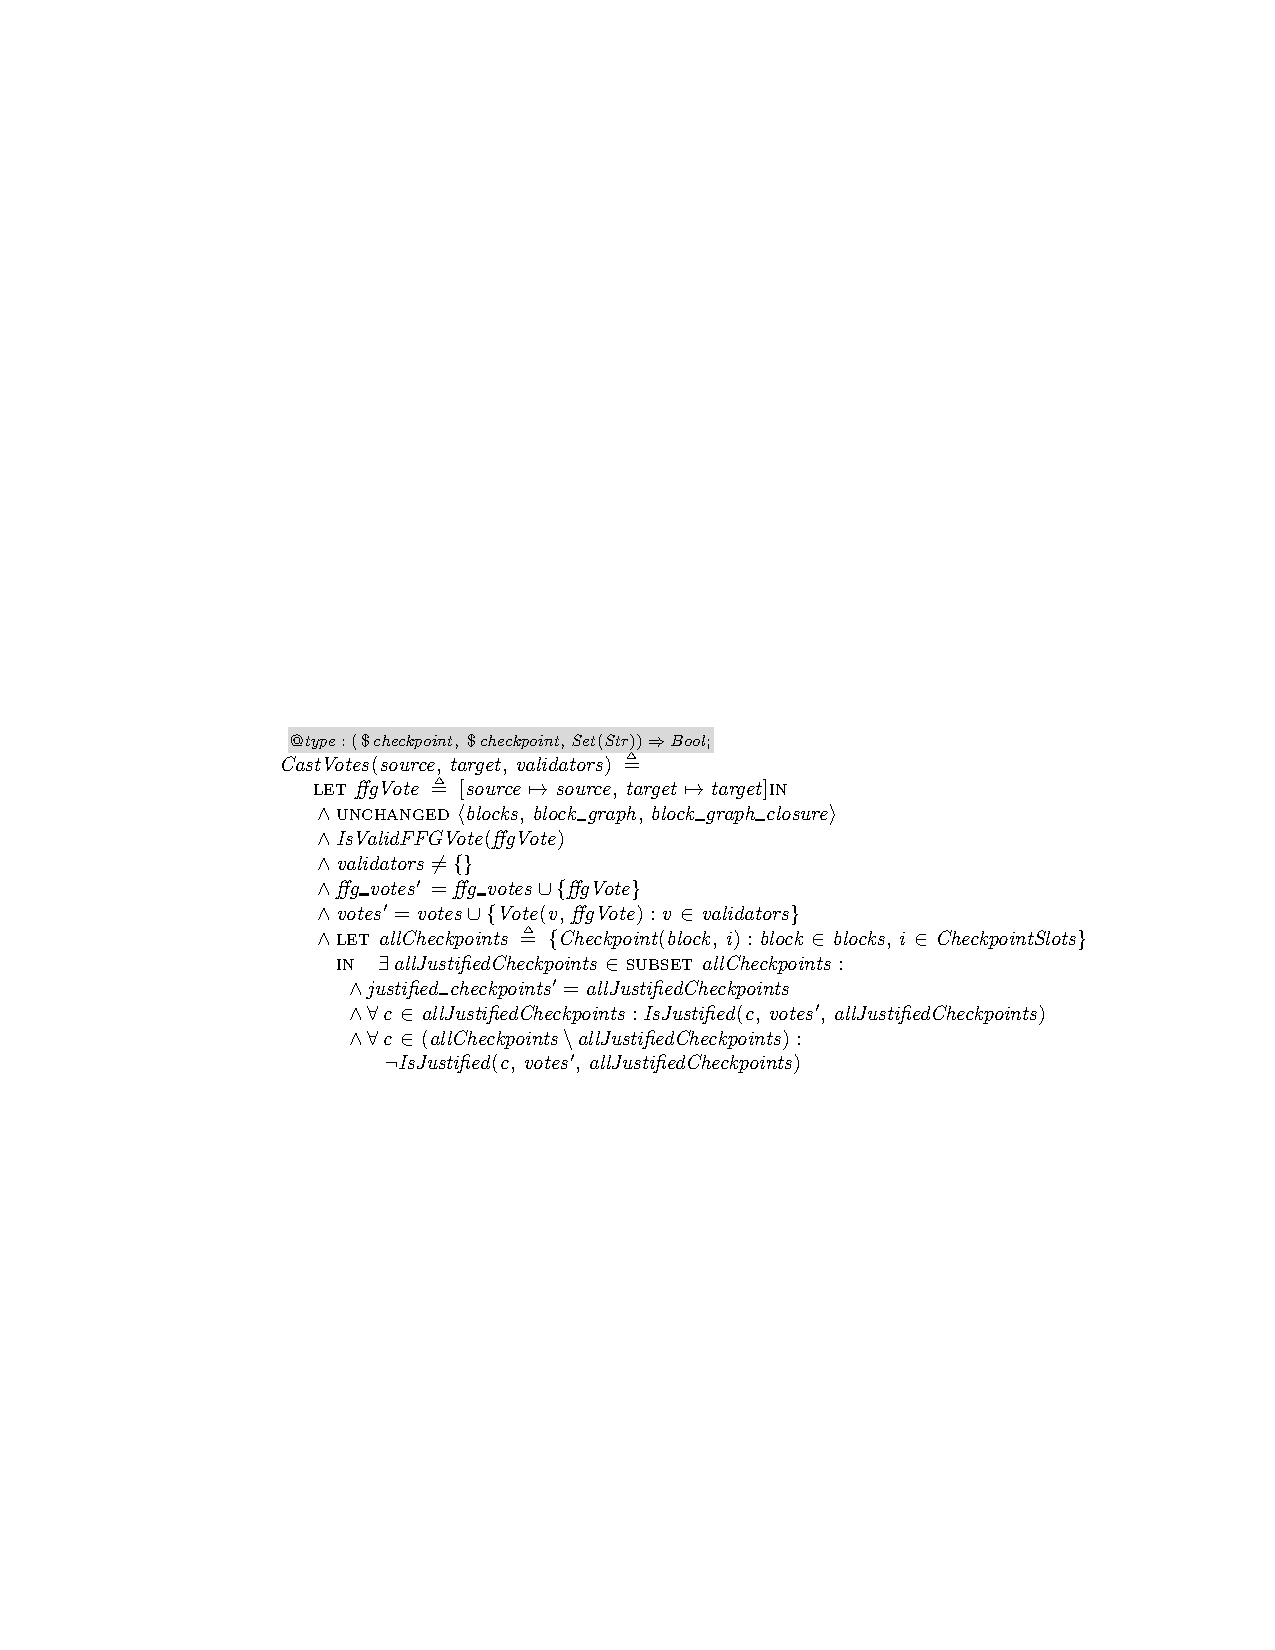
\includegraphics[width=\textwidth]{images/abstract-ffg-cast-votes.pdf}  % Include the PDF file
    \caption{A state-transition that casts votes}\label{fig:abstract-ffg-cast-votes}
\end{figure}

Figure~\ref{fig:abstract-ffg-next} shows the transition predicate of the
specification. It just non-deterministically chooses the inputs to
$\textit{ProposeBlock}$ or $\textit{CastVotes}$ and fires one of those two
actions.

\begin{figure}
    \centering
    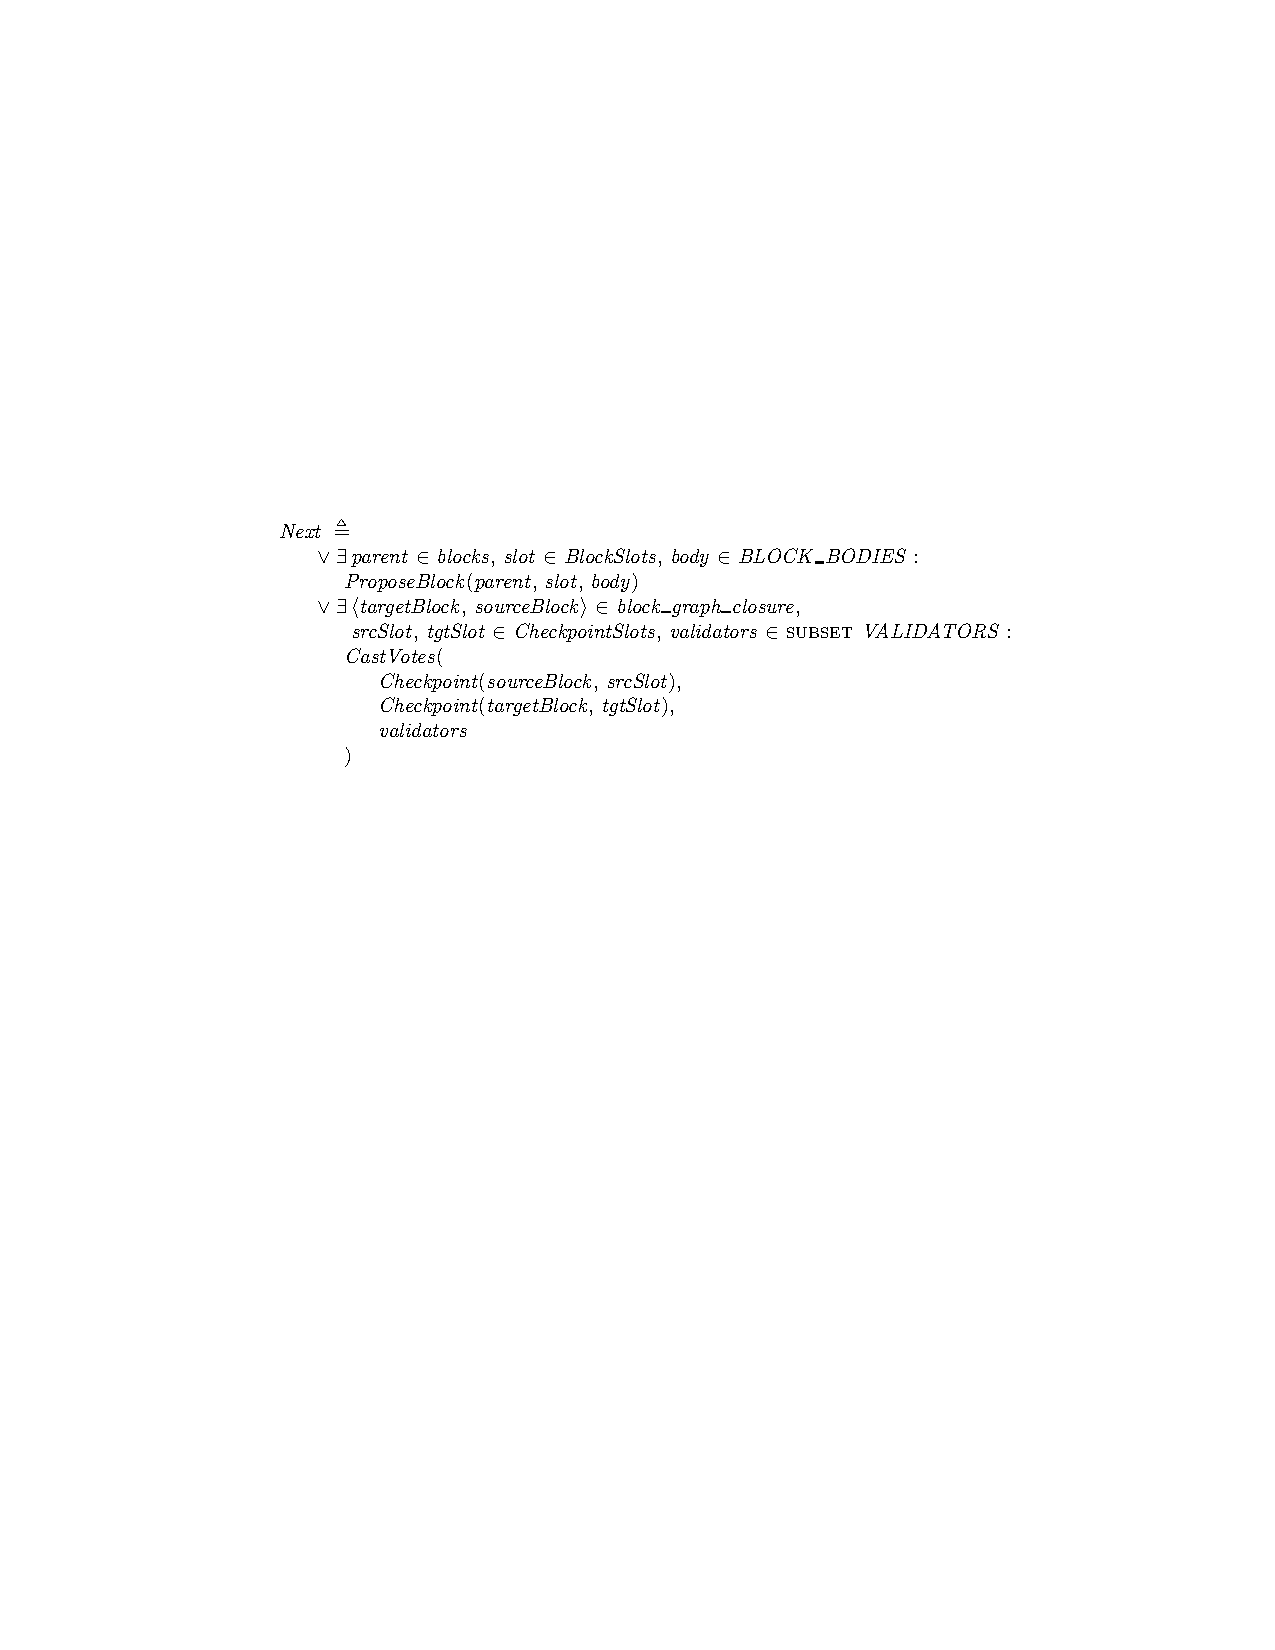
\includegraphics[width=\textwidth]{images/abstract-ffg-next.pdf}  % Include the PDF file
    \caption{The transition predicate of Spec 3}\label{fig:abstract-ffg-next}
\end{figure}

\paragraph{Model checking experiments.} We have conducted model checking
experiments with this specification. They are summarized in
Table~\ref{tab:abstract-ffg-mc}.

% 

\begin{table}
    \centering
    \begin{tabular}{llr}
        \tbh{State invariant}
            & \tbh{Command}
            & \tbh{Time}
            \\ \toprule
        $\textit{ExistsJustifiedNonGenesisInv}$
            & \texttt{check}
            & 5s
            \\ \midrule
        $\textit{ExistTwoFinalizedConflictingBlocks}$
            & \texttt{check}
            & 1h 27min
            \\ \midrule
        $\textit{AccountableSafety}$
            & \texttt{simulate}
            & N
            \\ \midrule
        $\textit{AccountableSafety}$
            & \texttt{check}
            & N
            \\ \bottomrule
    \end{tabular}
    \caption{Model checking experiments with Spec 3}\label{tab:abstract-ffg-mc}
\end{table}

